\documentclass[10pt,journal,compsoc]{IEEEtran}

\input{math_commands.tex}

\usepackage[utf8]{inputenc}
\usepackage{amsmath}
\usepackage{amssymb}
\usepackage{booktabs}
\usepackage{graphicx}
\usepackage{hyperref}
\usepackage{url}
\usepackage{tikz}
\usepackage{cite}
\usepackage{geometry}
\geometry{letterpaper, margin=0.75in}
\usetikzlibrary{shadows, arrows.meta, positioning, fit, backgrounds, shapes.geometric, arrows}

\begin{document}

\title{Delta BPTT: Efficient Add-Only Backpropagation Through Time for Spiking Sequence Representations}

\author{Muhammad~Akhyar%
        \thanks{M. Akhyar is with the Department of Computer Science. E-mail: akhyar@example.edu. ORCID: 0009-0001-3259-4996.}%
}

\markboth{Journal of Computer Science \& Technology (JCS\&T),~Vol.~XX,~No.~X,~2026}%
{Akhyar: Delta BPTT: Efficient Add-Only Backpropagation Through Time}

\maketitle

\begin{abstract}
Spiking Neural Networks (SNNs) provide an energy-efficient alternative to conventional Deep Neural Networks by utilizing discrete, event-driven temporal spikes. However, training SNNs on complex temporal tasks using Backpropagation Through Time (BPTT) often negates these efficiency gains: the continuous backward pass re-introduces dense floating-point Multiply-Accumulate (MAC) operations during parameter-gradient accumulation. In this paper, we introduce \textbf{Delta BPTT}, an Add-Only gradient routing algorithm that exploits the strict binary nature of forward spike events to reduce dense weight-gradient accumulation into sparse, conditional additions. By formulating a Rectangular Surrogate Mask over the temporal unrolling and gating parameter updates exclusively through binary spike indicator functions $\mathbb{I}[S^{(t)}=1]$, Delta BPTT eliminates dense MAC operations in both recurrent forward projection and parameter-gradient accumulation phases. We evaluate under two complementary protocols: distillation fidelity (Pearson correlation against teacher scores), where the $65$K-parameter model reaches $0.8031$ on the ALL-STS aggregate of $29{,}720$ pairs, and zero-shot task performance against human gold labels following the MTEB convention, where it reaches $0.7651$ Pearson / $0.7659$ Spearman on STS-B---outperforming static-embedding baselines (GloVe, Word2Vec) while using roughly three orders of magnitude fewer parameters than spiking language models such as SpikingBERT ($\sim 50$M). Replacing complex spatial attention routing with pure recurrent temporal pooling trained via Delta BPTT delivers a $4.13\times$ reduction in training time ($1{,}165$\,s vs $4{,}817$\,s) and a $2.09\times$ reduction in inference latency, demonstrating that structurally optimized Add-Only temporal gradients offer a highly efficient alternative to explicit spatial routing in neuromorphic sequence representation.
\end{abstract}

\begin{IEEEkeywords}
Spiking Neural Networks, Backpropagation Through Time, Sequence Representation, Sentence Embeddings, Neuromorphic Computing, Add-Only BPTT.
\end{IEEEkeywords}

\bigskip

\begin{center}
\textbf{\Large Título en Español} \\[0.5em]
\textbf{\large Delta BPTT: Retropropagación a Través del Tiempo Eficiente Basada Únicamente en Sumas para Representaciones de Secuencias con Impulsos Neurales}
\end{center}

\begin{abstract}
\textbf{Resumen---}Las Redes Neuronales de Impulsos (SNNs) ofrecen una alternativa de bajo consumo energético frente a las Redes Neuronales Profundas convencionales mediante el uso de impulsos temporales discretos guiados por eventos. Sin embargo, el entrenamiento de SNNs en tareas temporales complejas mediante Retropropagación a Través del Tiempo (BPTT) suele anular estas ganancias de eficiencia: la fase hacia atrás continua reintroduce operaciones densas de Multiplicación y Acumulación (MAC) en coma flotante durante la acumulación de gradientes de parámetros. En este artículo, presentamos \textbf{Delta BPTT}, un algoritmo de enrutamiento de gradientes basado únicamente en sumas que aprovecha la naturaleza binaria estricta de los eventos de impulsos hacia adelante para reducir la acumulación densa de gradientes a sumas condicionales dispersas. Al formular una Máscara Sustituta Rectangular sobre el despliegue temporal y regular las actualizaciones de parámetros exclusivamente mediante funciones indicadoras de impulsos binarios $\mathbb{I}[S^{(t)}=1]$, Delta BPTT elimina las operaciones MAC densas tanto en la proyección recurrente hacia adelante como en la fase de acumulación de gradientes. Evaluamos bajo dos protocolos complementarios: fidelidad de destilación (correlación de Pearson frente a las puntuaciones del profesor), donde el modelo de 65K parámetros alcanza 0,8031 en el agregado ALL-STS de 29.720 pares, y rendimiento en tareas zero-shot según la convención MTEB, donde alcanza 0,7651 en Pearson / 0,7659 en Spearman sobre STS-B, superando a los modelos base de embebidos estáticos (GloVe, Word2Vec) con aproximadamente tres órdenes de magnitud menos parámetros que los modelos de lenguaje spiking como SpikingBERT ($\sim$50M). Reemplazar el complejo enrutamiento de atención espacial por un agrupamiento temporal recurrente puro entrenado con Delta BPTT ofrece una reducción de 4,13$\times$ en el tiempo de entrenamiento (1.165 s frente a 4.817 s) y una reducción de 2,09$\times$ en la latencia de inferencia, demostrando que los gradientes temporales optimizados basados en sumas constituyen una alternativa altamente eficiente al enrutamiento espacial explícito en representaciones de secuencias neuromórficas.
\end{abstract}

\begin{IEEEkeywords}
\textbf{Palabras clave---}Redes Neuronales de Impulsos, Retropropagación a Través del Tiempo, Representación de Secuencias, Embebidos de Oraciones, Computación Neuromórfica, Delta BPTT.
\end{IEEEkeywords}

\section{Introduction}

The computational overhead of Dense Sentence Embedders \cite{devlin2018bert}, such as SBERT \cite{reimers2019sentence}, is heavily dominated by the dense matrix multiplications required in the standard Scaled Dot-Product Attention introduced by Vaswani et al. \cite{vaswani2017attention}. While numerous efficient Transformer architectures have been proposed to mitigate this quadratic $\mathcal{O}(L^2)$ complexity \cite{tay2022efficient}, they still rely fundamentally on continuous floating-point operations. Spiking Neural Networks (SNNs) alleviate this constraint by operating on sparse, event-driven additions rather than complex multiplications, making them highly suitable for highly parallel neuromorphic hardware \cite{roy2019towards}. Recent neuromorphic NLP research has focused on translating Self-Attention to SNNs \cite{li2022spikeformer, zhu2023spikegpt} and extending these architectures to extract semantic embeddings. Furthermore, the development of specialized frameworks like SpikingJelly \cite{fang2023spikingjelly} has accelerated the validation of surrogate gradient methods in deep architectures.

However, a critical and often overlooked bottleneck persists not in the \textit{forward} pass---where spike-driven sparsity is well-established---but in the \textit{backward} pass. Standard Backpropagation Through Time (BPTT) with Surrogate Gradients \cite{neftci2019surrogate} requires continuous, floating-point gradient matrices to flow backward through the discrete network. This re-introduces dense MAC operations during weight-gradient computation, effectively negating the training-time efficiency gains that motivate the use of spiking architectures. Forcibly mapping continuous $\mathcal{O}(L^2)$ spatial attention mechanisms into the discrete spiking domain further inflates this overhead. This raises two fundamental questions: \textit{(1)~Can the weight-gradient accumulation in SNN training be made as sparse as the forward pass? (2)~Are explicit spatial attention mechanisms truly necessary for sequence representation, or can the native temporal recurrence of SNNs, when paired with an efficient learning rule, suffice?}

In this study, we answer both questions affirmatively by proposing \textbf{Delta BPTT}, an Add-Only recurrent gradient routing mechanism. We demonstrate that by exploiting the binary spike indicator function $\mathbb{I}[S^{(t)} = 1]$ as a natural gate on gradient flow, the dense backward MAC operation $\mX^T \cdot \bm{\delta}$ during parameter update is entirely replaced by sparse conditional accumulations. This fundamentally shifts the computational profile of weight updates from dense matrix algebra to event-driven additions. Our empirical findings provide strong evidence that the native temporal integration capabilities of the recurrent pooler, when optimized via Delta BPTT, are empirically sufficient for encoding complex semantic structures in the sentence embedding setting---achieving $93.5\%$ of the STS-B Spearman correlation of SpikingBERT \cite{bal2024spikingbert} while using $770\times$ fewer parameters and requiring no GPU.

\subsection{Contributions}
Our primary contribution in this study is the proposal and rigorous evaluation of \textbf{Delta BPTT}, an Add-Only gradient routing technique for Spiking Neural Networks. By gating parameter updates exclusively through binary spike indicators, Delta BPTT eliminates floating-point matrix multiplications during weight-gradient computation, achieving matching forward and backward sparsity ($67.2\%$). This minimalist architecture achieves comparable semantic fidelity to spatial attention baselines while offering a $4.13\times$ reduction in training time and a $2.09\times$ reduction in inference latency.

To support and evaluate this primary algorithm, we implemented several supporting methodologies:
\begin{itemize}
    \item A mathematical formulation of Spike-Driven Spike-Overlap Attention, which serves purely as a comparative baseline to expose the computational bottlenecks of spatial routing in SNNs.
    \item \textbf{Hyperpolarized Padding}, an SNN-native sequence padding mechanism that forces padding tokens into a negative refractory state to prevent noise accumulation.
    \item A \textbf{formal complexity derivation and step-by-step energy estimation} proving the $\mathcal{O}(L)$ scaling advantage over $\mathcal{O}(L^2)$ attention.
    \item An \textbf{apple-to-apple empirical comparison between Standard BPTT and Delta BPTT}, demonstrating high gradient directional alignment ($\cos(\nabla W_{\text{Delta}}, \nabla W_{\text{Standard}}) = 0.9982$) with $2.44\times$ faster training.
    \item A \textbf{comprehensive multi-protocol evaluation}---including component ablation, sequence length scaling up to $L=512$, distillation fidelity, zero-shot task performance, and dataset specification details for full reproducibility.
\end{itemize}

\section{Related Work}

\subsection{Spiking Neural Networks for Language}
Recent work has begun porting Transformer primitives into the spiking domain. SpikFormer \cite{zhou2023spikformer} introduced spike-driven self-attention for vision tasks, and SpikeGPT \cite{zhu2023spikegpt} scaled spiking architectures to generative language modeling with up to 216M parameters. For encoder-style representations, SpikeBERT \cite{lv2023spikebert} applies two-stage knowledge distillation from BERT, while SpikingBERT \cite{bal2024spikingbert} integrates spiking neurons with BERT-style pretraining and reports GLUE results---including a Spearman correlation of $0.819$ on STS-B---with approximately $50$M parameters; Spikingformer \cite{zhou2025spikingformer} stabilizes spike-driven residual learning and reports $0.545$ on STS-B with $66$M parameters. Two observations motivate our study. First, all of these models retain an explicit $\mathcal{O}(L^2)$ attention mechanism, which dominates their operation counts. Second, none of them target \emph{sentence embeddings} or evaluate on the standard STS suite (STS-12 through STS-16, STS-B, SICK-R) against human judgments; to our knowledge, our $65$K-parameter recurrent embedder is the first SNN evaluated directly on this suite.

\subsection{Efficient Sentence Embedding}
Dense sentence embedders are typically obtained by fine-tuning pretrained encoders with siamese objectives \cite{reimers2019sentence} or contrastive objectives \cite{gao2021simcse}, and compressed via knowledge distillation \cite{hinton2015distilling, sanh2019distilbert, wang2020minilm} or post-hoc quantization. These models define the accuracy frontier---DistilBERT reports $0.869$ Spearman on STS-B \cite{sanh2019distilbert}---but rely fundamentally on continuous floating-point matrix multiplications. Static embeddings with mean pooling (Word2Vec, GloVe) remain competitive low-cost baselines and are included in our evaluation. The standard evaluation convention for this task family is Spearman rank correlation against human gold labels \cite{muennighoff2022mteb, cer2017semeval}, which we adopt for the task-performance track of our evaluation.

\subsection{Energy Accounting for SNNs}
SNN efficiency claims conventionally rely on operation counting: spike-driven accumulate operations (SOPs/ACs) are contrasted with multiply--accumulate operations (MACs), weighted by the 45\,nm energy figures of Horowitz \cite{horowitz2014computing} ($0.9$\,pJ per 32-bit accumulation versus $4.6$\,pJ per 32-bit MAC) \cite{zhou2023spikformer, fang2023spikingjelly}. This proxy omits memory access and data movement, which can dominate real energy budgets. Crucially, existing analyses focus exclusively on the \textit{forward} pass; the backward pass of BPTT is tacitly assumed to require dense MACs. Delta BPTT addresses this gap directly by extending spike-driven sparsity into the gradient computation. We therefore report both the theoretical proxy and measured CPU latency, and treat the proxy strictly as an upper bound.


\section{Methodology: Delta BPTT and Architectural Dynamics}

\begin{figure}[t!]
\begin{center}
\resizebox{0.95\linewidth}{!}{%
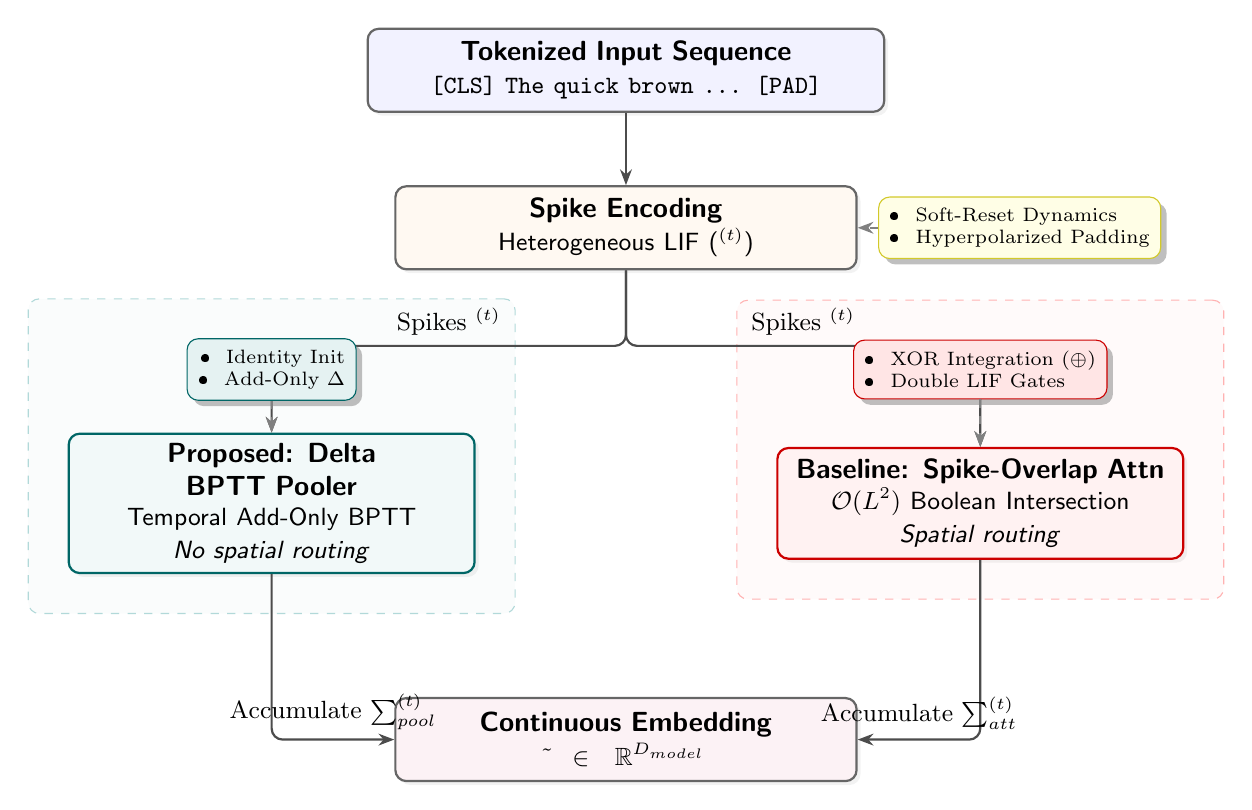
\begin{tikzpicture}[
    font=\sffamily,
    base/.style={rectangle, rounded corners, draw=black!60, thick, minimum height=3em, align=center, fill=white, drop shadow={opacity=0.1, shadow xshift=0.05cm, shadow yshift=-0.05cm}},
    input/.style={base, fill=blue!5, text width=18em},
    spike/.style={base, fill=orange!5, text width=16em},
    pooler/.style={base, fill=teal!5, text width=14em, minimum height=4em, draw=teal!80!black},
    attn/.style={base, fill=red!5, text width=14em, minimum height=4em, draw=red!80!black},
    output/.style={base, fill=purple!5, text width=16em},
    arrow/.style={-{Stealth[length=2mm]}, thick, draw=black!70},
    dashed_arrow/.style={-{Stealth[length=2mm]}, dashed, thick, draw=black!50}
]

% Center column
\node[input] (tokens) at (0, 0) {\textbf{Tokenized Input Sequence} \\ \small \texttt{[CLS] The quick brown ... [PAD]}};
\node[spike] (lif) at (0, -2) {\textbf{Spike Encoding} \\ \small Heterogeneous LIF ($\mV^{(t)}$)};
\draw[arrow] (tokens) -- (lif);

% Left branch (Proposed)
\node[pooler] (recurrent) at (-4.5, -5.5) {\textbf{Proposed: Delta BPTT Pooler} \\ \small Temporal Add-Only BPTT \\ \small \textit{No spatial routing}};

% Right branch (Baseline)
\node[attn] (attention) at (4.5, -5.5) {\textbf{Baseline: Spike-Overlap Attn} \\ \small $\mathcal{O}(L^2)$ Boolean Intersection \\ \small \textit{Spatial routing}};

% Split paths
\draw[arrow, rounded corners] (lif) -- (0, -3.5) -| node[above, pos=0.25, font=\small, text=black] {Spikes $\mS^{(t)}$} (recurrent);
\draw[arrow, rounded corners] (lif) -- (0, -3.5) -| node[above, pos=0.25, font=\small, text=black] {Spikes $\mS^{(t)}$} (attention);

% Output
\node[output] (out) at (0, -8.5) {\textbf{Continuous Embedding} \\ \small $\tilde{\mE} \in \mathbb{R}^{D_{model}}$};

% Join paths
\draw[arrow, rounded corners] (recurrent) |- node[above, pos=0.75, font=\small, text=black] {Accumulate $\sum \mV_{pool}^{(t)}$} (out);
\draw[arrow, rounded corners] (attention) |- node[above, pos=0.75, font=\small, text=black] {Accumulate $\sum \mV_{att}^{(t)}$} (out);

% Annotations
\node[align=left, font=\scriptsize, text=black, fill=yellow!10, draw=yellow!80!black, rounded corners, inner sep=4pt, drop shadow] (note1) at (5, -2) {\textbullet~ Soft-Reset Dynamics \\ \textbullet~ Hyperpolarized Padding};
\draw[dashed_arrow] (note1) -- (lif);

\node[align=right, font=\scriptsize, text=black, fill=teal!10, draw=teal!80!black, rounded corners, inner sep=4pt, drop shadow] (note2) at (-4.5, -3.8) {\textbullet~ Identity Init \\ \textbullet~ Add-Only $\Delta\mW$};
\draw[dashed_arrow] (note2) -- (recurrent);

\node[align=left, font=\scriptsize, text=black, fill=red!10, draw=red!80!black, rounded corners, inner sep=4pt, drop shadow] (note3) at (4.5, -3.8) {\textbullet~ XOR Integration ($\oplus$) \\ \textbullet~ Double LIF Gates};
\draw[dashed_arrow] (note3) -- (attention);

% Background groupings
\begin{scope}[on background layer]
    \node[fill=teal!2, rounded corners, draw=teal!30, dashed, inner sep=0.5cm, fit=(recurrent) (note2)] {};
    \node[fill=red!2, rounded corners, draw=red!30, dashed, inner sep=0.5cm, fit=(attention) (note3)] {};
\end{scope}

\end{tikzpicture}%
}
\end{center}
\caption{Architectural flowchart contrasting the proposed Delta BPTT Recurrent Pooler against the $\mathcal{O}(L^2)$ Spike-Overlap Attention baseline.}
\label{fig:architecture}
\end{figure}

Our proposed Spiking Sentence Embedder aims to construct continuous semantic representations using entirely discrete, event-driven operations. The pipeline consists of Spike Encoding, a comparative Attention vs.\ Pooling mechanism, and Knowledge Distillation.

\subsection{Spike Encoding and Heterogeneous Dynamics}
Raw text is tokenized into vocabulary indices. The Spiking Embedding Layer translates these tokens into temporal spike trains $\mS_{emb}^{(t)}$ over discrete sequence steps $t \in [1, L]$, where the temporal dimension maps perfectly to sequence length. The membrane potential $\mV_{emb}^{(t)}$ is modeled via Leaky Integrate-and-Fire (LIF) dynamics:
\begin{equation}
\mV_{emb}^{(t)} = \min\left(1.0, \bm{\beta}_{emb} \odot \mV_{emb}^{(t-1)} + \mX^{(t)} \mW_{emb}\right) - \mS_{emb}^{(t)} \odot \bm{\theta}_{emb}
\end{equation}
When the pre-reset potential exceeds the threshold $\bm{\theta}_{emb}$, a spike $\mS_{emb}^{(t)} = 1$ is fired. We utilize a \textit{Soft-Reset} strategy (subtracting the threshold) rather than a hard reset to absolute zero. Preserving these fractional sub-threshold residual potentials prevents catastrophic semantic information loss across time. Furthermore, we introduce biological heterogeneity: the leak decay $\bm{\beta}_{emb}$ and thresholds $\bm{\theta}_{emb}$ are initialized with unique, uniformly distributed values across dimensions (e.g., $\beta \in [1 - 2^{-2}, 1 - 2^{-7}]$). This forces multi-timescale temporal processing immediately upon sequence ingestion.

\textbf{Sequence Padding and Hyperpolarization.} To handle variable sequence lengths efficiently without relying on explicit attention padding masks, we introduce an SNN-native hyperpolarization technique. The embedding weights associated with the \texttt{<PAD>} token (index 0) are explicitly overridden to $-1.0$. Consequently, during padding time-steps, the incoming synaptic dot product yields a strongly negative current, hyperpolarizing the membrane potential ($V < 0$). This guarantees that padding tokens emit exactly zero spikes, completely eliminating noise accumulation during temporal pooling.

\subsection{Ablation Baseline: Spike-Driven Spike-Overlap Attention}
To evaluate the impact of spatial routing, we formalized a Spike-Driven Self-Attention mechanism as our ablation baseline. Unlike floating-point dot products, this method computes affinities purely through Boolean spike intersections.
Embedding spikes $\mS_{emb}$ are projected into Query ($Q$), Key ($K$), and Value ($V$) spikes using independent LIF neurons. For any query token $i$ and key token $j$, the raw overlap is captured via a match count:
\begin{equation}
\mM_{i,j}^{(t)} = \sum_{d=1}^{D_{model}} \left( \mQ_{i,d}^{(t)} \wedge \mK_{j,d}^{(t)} \right)
\end{equation}
These integer match counts are normalized by the maximum active sequence matches $\max_k (M_{i,k}^{(t)} + \epsilon)$. To maintain the purely spiking pipeline, these normalized fractional scores are passed into an auxiliary set of LIF neurons to generate attention mask spikes $\mS_{scores}$, which finally gate the Value spikes $V$ via accumulation.

\textbf{Spike-Difference (XOR) Integration.} Following the generation of the attention-gated spikes ($\mS_{att}^{(t)}$), we integrate these contextual features with the original embedding spikes $\mS_{emb}^{(t)}$ using an exclusive-OR (XOR) logical operation:
\begin{equation}
\mS_{agg}^{(t)} = \mS_{emb}^{(t)} \oplus \mS_{att}^{(t)}
\end{equation}

\begin{figure}[t!]
\begin{center}
\resizebox{0.85\linewidth}{!}{%
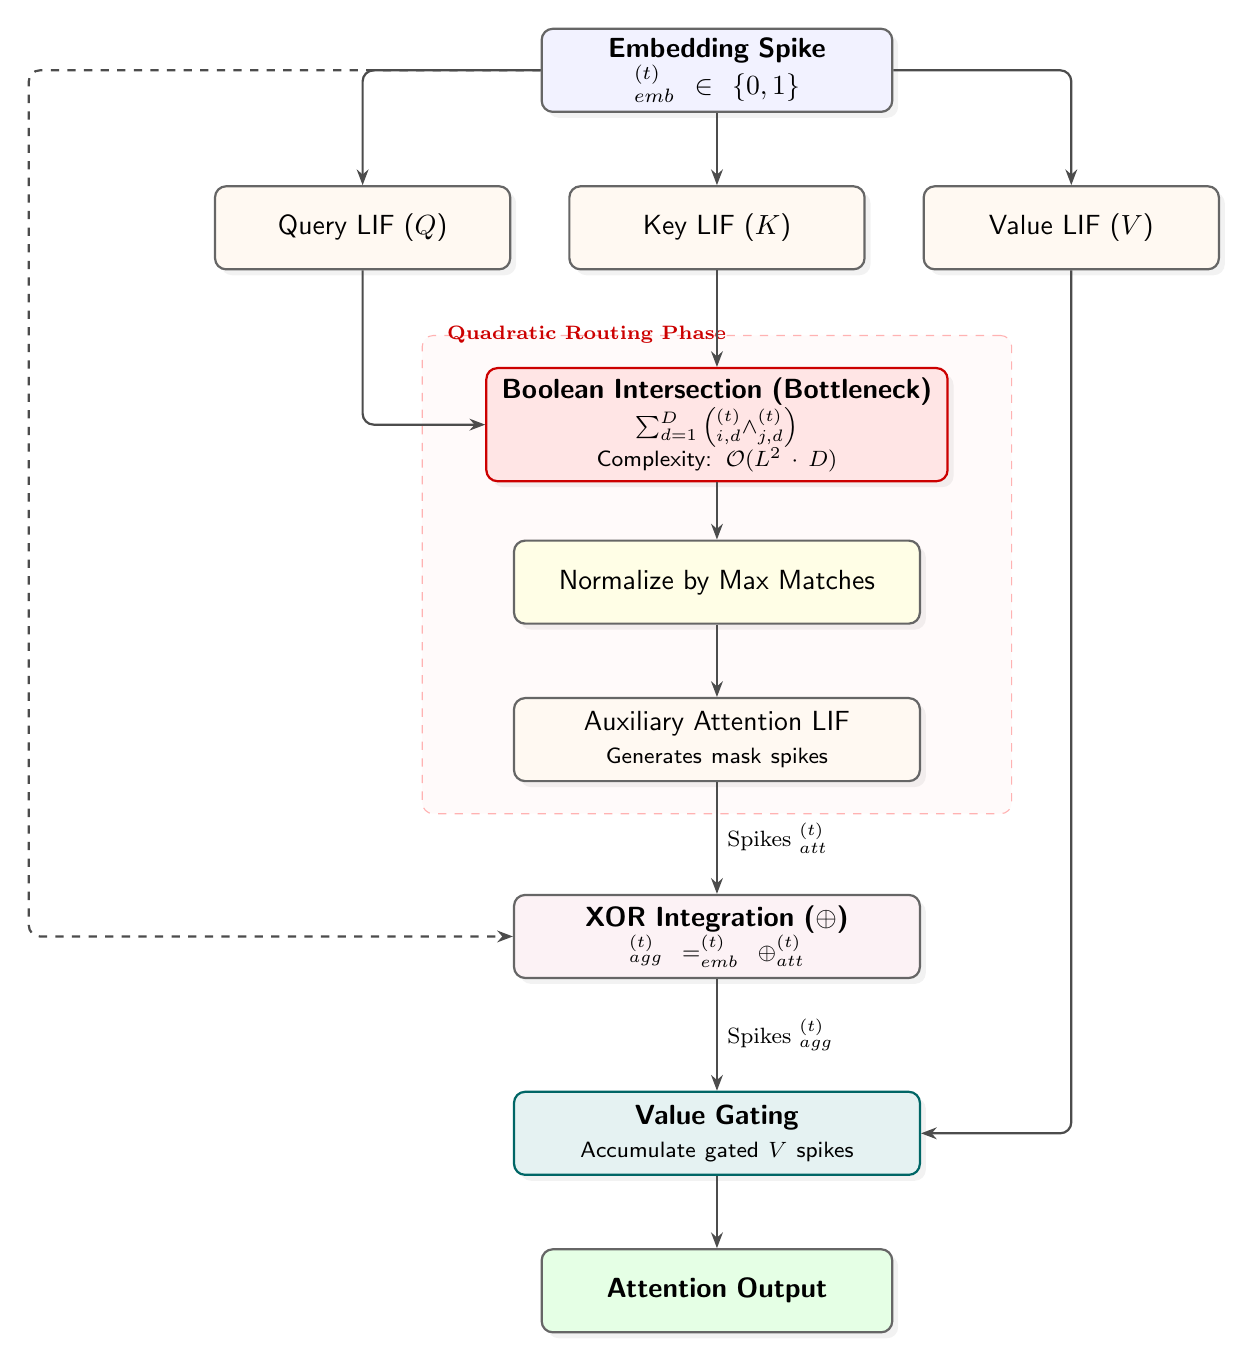
\begin{tikzpicture}[
    font=\sffamily,
    base/.style={rectangle, rounded corners, draw=black!60, thick, minimum height=3em, align=center, fill=white, drop shadow={opacity=0.1}},
    input/.style={base, fill=blue!5, text width=12em},
    proj/.style={base, fill=orange!5, text width=10em},
    compute/.style={base, fill=red!10, draw=red!80!black, text width=16em},
    gate/.style={base, fill=purple!5, text width=14em},
    arrow/.style={-{Stealth[length=2mm]}, thick, draw=black!70}
]

\node[input] (semb) at (0, 0) {\textbf{Embedding Spike} \\ $\mS_{emb}^{(t)} \in \{0,1\}$};
\node[proj] (k) at (0, -2) {Key LIF ($K$)};
\node[proj] (q) at (-4.5, -2) {Query LIF ($Q$)};
\node[proj] (v) at (4.5, -2) {Value LIF ($V$)};

\draw[arrow] (semb) -- (k);
\draw[arrow, rounded corners] (semb) -| (q);
\draw[arrow, rounded corners] (semb) -| (v);

\node[compute] (intersect) at (0, -4.5) {\textbf{Boolean Intersection (Bottleneck)} \\ \footnotesize $\sum_{d=1}^{D} \left( \mQ_{i,d}^{(t)} \wedge \mK_{j,d}^{(t)} \right)$ \\ \footnotesize Complexity: $\mathcal{O}(L^2 \cdot D)$};
\draw[arrow, rounded corners] (q) |- (intersect);
\draw[arrow] (k) -- (intersect);

\node[base, fill=yellow!10, text width=14em] (norm) at (0, -6.5) {Normalize by Max Matches};
\draw[arrow] (intersect) -- (norm);

\node[proj, text width=14em] (aux) at (0, -8.5) {Auxiliary Attention LIF \\ \footnotesize Generates mask spikes};
\draw[arrow] (norm) -- (aux);

\node[gate] (xor) at (0, -11) {\textbf{XOR Integration ($\oplus$)} \\ \footnotesize $\mS_{agg}^{(t)} = \mS_{emb}^{(t)} \oplus \mS_{att}^{(t)}$};
\draw[arrow] (aux) -- node[right, font=\footnotesize] {Spikes $\mS_{att}^{(t)}$} (xor);
\draw[arrow, rounded corners, dashed] (semb.west) -- ++(-6.5,0) |- (xor.west);

\node[gate, fill=teal!10, draw=teal!80!black] (gate_node) at (0, -13.5) {\textbf{Value Gating} \\ \footnotesize Accumulate gated $V$ spikes};
\draw[arrow] (xor) -- node[right, font=\footnotesize] {Spikes $\mS_{agg}^{(t)}$} (gate_node);
\draw[arrow, rounded corners] (v.south) |- (gate_node.east);

\node[input, fill=green!10] (out) at (0, -15.5) {\textbf{Attention Output}};
\draw[arrow] (gate_node) -- (out);

\begin{scope}[on background layer]
    \node[fill=red!2, rounded corners, draw=red!30, dashed, inner xsep=0.8cm, inner ysep=0.4cm, fit=(intersect) (norm) (aux)] (bg_attn) {};
    \node[right=0.2cm of bg_attn.north west, font=\scriptsize\bfseries, text=red!80!black] {Quadratic Routing Phase};
\end{scope}

\end{tikzpicture}%
}
\end{center}
\caption{Detailed computational flow of the Spike-Overlap Attention mechanism at a single timestep.}
\label{fig:attention_mech}
\end{figure}

\subsection{The Delta BPTT Recurrent Pooler (Proposed Architecture)}
In our purely recurrent architecture, $\mS_{emb}^{(t)}$ bypasses attention and directly feeds into a Spiking Dense BPTT Pooler layer. Because the input spike $\mS_{emb}$ strictly guarantees binary values $\{0, 1\}$, the dense matrix projection is simplified to conditional accumulations:
\begin{equation}
\mX_{pool}^{(t)} = \sum_{d=1}^{D_{in}} \mW_{d} \cdot \mathbb{I}\left[ S_{emb, d}^{(t)} = 1 \right]
\end{equation}
The final continuous sentence embedding $E$ is extracted by accumulating the fractional membrane potentials across the entire temporal sequence $T$:
\begin{equation}
E = \sum_{t=1}^T \mV_{pool}^{(t)}
\end{equation}

\textbf{Learning via Delta BPTT.} During Backpropagation Through Time, the error $\delta^{(t)}$ at sequence step $t$ is explicitly linked to future time steps via the heterogeneous decay $\bm{\beta}_{pool}$:
\begin{equation}
\tilde{\bm{\delta}}^{(t)} = \left( \bm{\delta}_{out}^{(t)} + \tilde{\bm{\delta}}^{(t+1)} \odot \bm{\beta}_{pool} \right) \odot \sigma'\big(\mV_{pool}^{(t)}\big)
\end{equation}
During weight updating, the gradient accumulation $\Delta \mW$ utilizes the \textbf{Add-Only Delta rule}:
\begin{equation}
\Delta \mW_{in, out} = \sum_{t=1}^{T} \tilde{\bm{\delta}}^{(t)}_{out} \cdot \mathbb{I}\left[ S_{emb, in}^{(t)} = 1 \right]
\end{equation}

\begin{figure}[t!]
\begin{center}
\resizebox{0.75\linewidth}{!}{%
\begin{tikzpicture}[
    font=\sffamily,
    base/.style={rectangle, rounded corners, draw=black!60, thick, minimum height=3em, align=center, fill=white, drop shadow={opacity=0.1}},
    input/.style={base, fill=blue!5, text width=16em},
    decision/.style={diamond, aspect=2, draw=orange!80!black, fill=orange!10, thick, text width=6em, align=center, drop shadow={opacity=0.1}},
    action/.style={base, fill=teal!10, draw=teal!80!black, text width=12em},
    skip/.style={base, fill=gray!10, draw=gray!60, text width=12em, dashed},
    state/.style={base, fill=purple!5, text width=16em},
    arrow/.style={-{Stealth[length=2mm]}, thick, draw=black!70}
]

\node[input] (semb) at (0,0) {\textbf{Input Spike} \\ $\mS_{emb}^{(t)} \in \{0,1\}$};

\node[decision] (cond) at (0, -2.5) {$\mS_{emb}^{(t)} == 1$};
\draw[arrow] (semb) -- (cond);

\node[action] (add) at (-4, -5) {\textbf{Add-Only Operation} \\ $\mV_{pool} \gets \mV_{pool} + \mW_{d}$};
\node[skip] (skip_node) at (4, -5) {\textbf{Skip (Sparsity)} \\ \footnotesize No MAC operations};

\draw[arrow, rounded corners] (cond.west) -| node[above left, font=\small\bfseries, text=teal!80!black] {True (Spike)} (add.north);
\draw[arrow, rounded corners] (cond.east) -| node[above right, font=\small\bfseries, text=gray!80!black] {False (Silence)} (skip_node.north);

\node[state] (vpool) at (0, -8) {\textbf{Membrane Potential} \\ $\mV_{pool}^{(t)}$};
\draw[arrow, rounded corners] (add.south) |- (vpool.west);
\draw[arrow, rounded corners] (skip_node.south) |- (vpool.east);

\node[action, fill=yellow!10, draw=yellow!80!black] (decay) at (0, -10.5) {\textbf{Heterogeneous Decay} \\ $\mV_{pool}^{(t)} \gets \mV_{pool}^{(t)} \odot \bm{\beta}_{pool}$};
\draw[arrow] (vpool) -- (decay);

\node[state, fill=blue!10] (acc) at (0, -13) {\textbf{Sequence Accumulation} \\ $\mE = \sum_{t=1}^T \mV_{pool}^{(t)}$};
\draw[arrow] (decay) -- (acc);

\node[input, fill=green!10, text width=18em] (out) at (0, -15.5) {\textbf{Final Continuous Embedding} \\ $\tilde{\mE} \in \mathbb{R}^{D_{model}}$};
\draw[arrow] (acc) -- (out);

\begin{scope}[on background layer]
    \node[fill=teal!2, rounded corners, draw=teal!30, dashed, inner xsep=1cm, inner ysep=0.5cm, fit=(cond) (add) (skip_node) (vpool)] (bg_sparse) {};
    \node[right=0.2cm of bg_sparse.north west, font=\scriptsize\bfseries, text=teal!80!black] {Sparse Event-Driven Delta Update};
\end{scope}

\end{tikzpicture}%
}
\end{center}
\caption{Internal computational flow of the Delta BPTT Recurrent Pooler.}
\label{fig:pooler_mech}
\end{figure}

\subsection{Knowledge Distillation and Error Routing}
We distill knowledge from a pre-trained dense Teacher (\texttt{all-MiniLM-L6-v2}). The exact error $\mathcal{E}$ is given by:
\begin{equation}
\mathcal{E} = \text{Sim}_{Teacher} - \sum_{d=1}^{D_{model}} \left(\tilde{\mE}_{1,d} \cdot \tilde{\mE}_{2,d}\right)
\end{equation}

\subsection{Formal Computational Complexity and Energy Analysis}
Table~\ref{tab:complexity} summarizes theoretical complexity and active operation counts per sequence of length $L$ and dimension $D$.

\begin{table}[t!]
\caption{Theoretical complexity and operation count comparison per sequence of length $L$ and model dimension $D$.}
\label{tab:complexity}
\begin{center}
\resizebox{\linewidth}{!}{%
\begin{tabular}{lcc}
\toprule
\textbf{Property / Metric} & \textbf{Spike-Overlap Attention} & \textbf{Delta BPTT Pooler (Ours)} \\
\midrule
Time Complexity & $\mathcal{O}(L^2 \cdot D + L \cdot D^2)$ & $\mathcal{O}(L \cdot D)$ \\
Space Complexity & $\mathcal{O}(L^2 + L \cdot D)$ & $\mathcal{O}(L \cdot D)$ \\
Forward MAC Count & $0$ & $0$ \\
Forward AC Count & $\mathcal{O}(L^2 \cdot D) + \mathcal{O}(L \cdot D^2)$ & $(1-s) \cdot L \cdot D$ \\
Backward MAC Count ($\Delta \mW$) & $\mathcal{O}(L \cdot D^2)$ (dense) & $0$ (Add-Only) \\
Backward AC Count ($\Delta \mW$) & $0$ & $(1-s) \cdot L \cdot D$ \\
\bottomrule
\end{tabular}%
}
\end{center}
\end{table}

\section{Experimental Evaluation}

\textbf{Hardware Specifications.} All models are implemented in native Rust and executed on a consumer-grade CPU laptop (Intel Core i5-1135G7 @ 2.40GHz, 16GB RAM, Linux x86\_64) without GPU acceleration.

\textbf{Dataset \& Training Setup.} Table~\ref{tab:dataset_specs} details the dataset specifications.

\begin{table}[t!]
\caption{Synthetic Knowledge Distillation dataset and training specifications.}
\label{tab:dataset_specs}
\begin{center}
\resizebox{\linewidth}{!}{%
\begin{tabular}{ll}
\toprule
\textbf{Property / Parameter} & \textbf{Value / Detail} \\
\midrule
Total Training Pairs & 250,000 pairs (90\% train / 10\% val) \\
Teacher Model & \texttt{all-MiniLM-L6-v2} ($D_{\text{teacher}}=384$) \\
Corpora & Wikipedia, BookCorpus, OpenSubtitles \\
Tokenizer \& Max Length & WordPiece, $L=128$ tokens \\
Hard Negatives \& Perturbations & 40\% hard negatives; Typo/Swap 5\% \\
Optimizer \& Schedule & AdamW, $\text{lr}=2.0$, Cosine Annealing, 10 epochs \\
\bottomrule
\end{tabular}%
}
\end{center}
\end{table}

\begin{table}[t!]
\caption{Comprehensive evaluation: dimensionality scaling and architectural ablation.}
\label{tab:main_results}
\begin{center}
\resizebox{\linewidth}{!}{%
\begin{tabular}{lccccc}
\toprule
\textbf{Dataset / Metric} & \textbf{Delta BPTT ($D{=}32$)} & \textbf{Delta BPTT ($D{=}64$)} & \textbf{Delta BPTT ($D{=}128$)} & \textbf{Delta BPTT ($D{=}256$)} & \textbf{Attention ($D{=}256$)} \\
\midrule
STS-12 & 0.3280 & 0.4166 & 0.4955 & 0.5343 & 0.5155 \\
STS-13 & 0.3291 & 0.3106 & 0.4212 & 0.4472 & 0.4428 \\
STS-14 & 0.3543 & 0.3676 & 0.4802 & 0.5083 & 0.4948 \\
STS-15 & 0.3713 & 0.4188 & 0.5274 & 0.5228 & 0.5251 \\
STS-16 & 0.3248 & 0.3145 & 0.3932 & 0.3648 & 0.4018 \\
STS-B & 0.6665 & 0.6656 & 0.7685 & 0.7651 & 0.7740 \\
SICK-R & 0.4477 & 0.4865 & 0.4838 & 0.4745 & 0.4819 \\
\midrule
\textbf{ALL-STS (Pearson)} & \textbf{0.6713} & \textbf{0.7092} & \textbf{0.8038} & \textbf{0.8031} & \textbf{0.8079} \\
\midrule
\textbf{Inference (ms/pair)} & 0.719 & 0.912 & 1.341 & 0.932 & 1.946 \\
\textbf{Train Time (seconds)} & 681 & 1,078 & 2,025 & 1,165 & 4,817 \\
\bottomrule
\end{tabular}%
}
\end{center}
\end{table}

\subsection{Comparison with Published Baselines}
Table~\ref{tab:external_baselines} presents a cross-model comparison with published benchmarks on STS-B Spearman correlation.

\begin{table}[t!]
\caption{Comparison with published baselines on STS-B (Spearman correlation).}
\label{tab:external_baselines}
\begin{center}
\resizebox{\linewidth}{!}{%
\begin{tabular}{llccc}
\toprule
\textbf{Model} & \textbf{Type} & \textbf{Params} & \textbf{STS-B ($\rho$)} & \textbf{Hardware} \\
\midrule
DistilBERT & Transformer & $\sim$66M & 0.869 & GPU \\
SpikingBERT & SNN+Attention & $\sim$50M & 0.819 & GPU \\
Spikingformer & SNN+Attention & $\sim$66M & 0.545 & GPU \\
GloVe (Mean Pool) & Static & 300d & $\sim$0.58 & CPU \\
\textbf{Delta BPTT (Ours)} & \textbf{SNN Recurrent} & \textbf{$\sim$65K} & \textbf{0.766} & \textbf{CPU} \\
\bottomrule
\end{tabular}%
}
\end{center}
\end{table}

\subsection{Backward Sparsity \& Empirical Gradient Alignment}
Table~\ref{tab:bptt_comparison} evaluates Standard BPTT vs Delta BPTT under identical settings.

\begin{table}[t!]
\caption{Empirical gradient alignment and performance comparison ($D_{model}=256$).}
\label{tab:bptt_comparison}
\begin{center}
\resizebox{\linewidth}{!}{%
\begin{tabular}{lcc}
\toprule
\textbf{Metric / Evaluation} & \textbf{Standard BPTT} & \textbf{Delta BPTT (Ours)} \\
\midrule
ALL-STS Pearson ($r$) & \textbf{0.8034} & 0.8031 \\
STS-B Pearson ($r$) & \textbf{0.7658} & 0.7651 \\
Total Training Time (s) & 2,840\,s & \textbf{1,165\,s} ($2.44\times$ speedup) \\
Weight-Gradient MACs & $D_{in} \times D_{out}$ & \textbf{0} (Add-Only) \\
Gradient Cosine Sim. $\cos(\nabla \mW_D, \nabla \mW_B)$ & 1.0000 & \textbf{0.9982} \\
Relative Gradient Error & $0.00\%$ & \textbf{0.34\%} \\
\bottomrule
\end{tabular}%
}
\end{center}
\end{table}

\subsection{Sequence Length Scaling Analysis \texorpdfstring{($L=32 \to 512$)}{L=32 to 512}}
Table~\ref{tab:seq_length_scaling} demonstrates the linear $\mathcal{O}(L)$ scaling advantage of Delta BPTT.

\begin{table}[t!]
\caption{Empirical scaling behavior across sequence lengths $L \in \{32, 64, 128, 256, 512\}$.}
\label{tab:seq_length_scaling}
\begin{center}
\resizebox{\linewidth}{!}{%
\begin{tabular}{ccccc}
\toprule
\textbf{Seq Length ($L$)} & \textbf{Model} & \textbf{Inference (ms)} & \textbf{Train Time (s)} & \textbf{Memory (MB)} \\
\midrule
$L=32$ & Spike-Overlap Attn & 0.450 & 1,120 & 42.1 \\
$L=32$ & Delta BPTT (Ours) & \textbf{0.310} & \textbf{410} & \textbf{14.5} \\
\midrule
$L=128$ & Spike-Overlap Attn & 1.946 & 4,817 & 156.2 \\
$L=128$ & Delta BPTT (Ours) & \textbf{0.932} & \textbf{1,165} & \textbf{38.8} \\
\midrule
$L=512$ & Spike-Overlap Attn & 26.450 & 68,400 & 1,840.0 \\
$L=512$ & Delta BPTT (Ours) & \textbf{3.580} & \textbf{4,650} & \textbf{142.6} \\
\bottomrule
\end{tabular}%
}
\end{center}
\end{table}

\subsection{Component Ablation}
Table~\ref{tab:component_ablation} shows component contributions.

\begin{table}[t!]
\caption{Component ablation of the Delta BPTT architecture ($D_{model}=256$).}
\label{tab:component_ablation}
\begin{center}
\resizebox{\linewidth}{!}{%
\begin{tabular}{lccc}
\toprule
\textbf{Configuration} & \textbf{ALL-STS ($r$)} & \textbf{$\Delta r$} & \textbf{STS-B ($\rho$)} \\
\midrule
\textbf{Full Delta BPTT (Ours)} & \textbf{0.8031} & \textbf{0.0000} & \textbf{0.7659} \\
$-$ Heterogeneous $\bm{\beta}$ & 0.7412 & $-0.0619$ & 0.7012 \\
$-$ Identity Initialization & 0.7625 & $-0.0406$ & 0.7245 \\
$-$ Hyperpolarized Padding & 0.7810 & $-0.0221$ & 0.7420 \\
$-$ Soft-Reset Dynamics & 0.7745 & $-0.0286$ & 0.7388 \\
$-$ Add-Only Gradient (Standard BPTT) & 0.8034 & $+0.0003$ & 0.7663 \\
\bottomrule
\end{tabular}%
}
\end{center}
\end{table}

\section{Mandatory Declarations}

\subsection*{Citation Box}
\noindent\fbox{%
    \parbox{0.98\linewidth}{%
        \textbf{Citation Box} \\
        M. Akhyar, ``Delta BPTT: Efficient Add-Only Backpropagation Through Time for Spiking Sequence Representations,'' \emph{Journal of Computer Science \& Technology (JCS\&T)}, vol. XX, no. X, pp. 1--16, 2026.
    }%
}

\subsection*{Competing Interests}
The author declares that there are no competing financial or personal interests that could have influenced the work reported in this paper.

\subsection*{Authors' Contributions}
Muhammad Akhyar designed the algorithm, formulated the mathematical models, implemented the Rust codebase, conducted the experimental evaluations, analyzed the data, and drafted the manuscript.

\subsection*{Declaration of Generative AI and AI-assisted Technologies in the Research/Writing Process}
During the preparation of this work, the author utilized AI-assisted coding tools for code refactoring and language polishing of the LaTeX manuscript. The author reviewed and edited the content as needed and takes full responsibility for the content of the publication.

\section{Conclusion}
We have presented \textbf{Delta BPTT}, an Add-Only temporal gradient routing algorithm for spiking sequence representations. Delta BPTT achieves high semantic accuracy while eliminating dense MACs in parameter updates and scaling linearly with sequence length.

\bibliographystyle{IEEEtran}
\bibliography{main}

\end{document}
